\subsubsection{usergoal-ugWitnessSendFamilyNotification}

\label{RE-use-case-ugWitnessSendFamilyNotification}




\begin{usecase}
  \addheading{Use-Case Description}
  \addsingletwocolumnrow{Name}{ugWitnessSendFamilyNotification}
  \addsingletwocolumnrow{Scope}{system}
  \addsingletwocolumnrow{Level}{usergoal}
  

\addrowheading{Primary actor(s)}
\addnumberedsinglerow{}{\msrcode{actSystem[active]}}


\addrowheading{Secondary actor(s)}
\addnumberedsinglerow{}{\msrcode{actAuthenticated[active]}}
\addnumberedsinglerow{}{\msrcode{actCoordinator[proactive]}}

\addrowheading{Goal(s) description}
\addsinglerow{}

\addrowheading{Reuse}
\addnumberedsinglerow{}{\msrucname{oeCreateAlert [1..*]}}
\addnumberedsinglerow{}{\msrucname{oeCreateCrisis [1..1]}}
\addnumberedsinglerow{}{\msrucname{oeUpdateCrisis [0..*]}}

\addrowheading{Protocol condition(s)}
\addnumberedsinglerow{}{
}

\addrowheading{Pre-condition(s)}
\addnumberedsinglerow{}{
}

\addrowheading{Main post-condition(s)}
\addnumberedsinglerow{}{
}

\addrowheading{Main Steps}
\addalphanumberedsinglerow{}{the actor \msrcode{actAuthenticated} executes the \msrucname{oeCreateAlert} use case}
\addalphanumberedsinglerow{}{the actor \msrcode{actCoordinator} executes the \msrucname{oeCreateAlert} use case}
\addalphanumberedsinglerow{}{the actor \msrcode{actCoordinator} executes the \msrucname{oeCreateCrisis} use case}
\addalphanumberedsinglerow{}{the actor \msrcode{actSystem} executes the \msrucname{oeChooseInformation} use case}
\addalphanumberedsinglerow{}{the actor \msrcode{actCoordinator} executes the \msrucname{oeUpdateCrisis} use case}
\addrowheading{Steps Ordering Constraints}
\addnumberedsinglerow{}{if c then previously a or b}
\addnumberedsinglerow{}{if d then previously a or b}
\addnumberedsinglerow{}{if e then previously a or b}

\addrowheading{Additional Information}
\addsinglerow{
none
}

\end{usecase} 


Figure \ref{fig:lu.uni.lassy.excalibur.examples.icrash-RE-UCD-uc-ugWitnessSendFamilyNotification}
The authenticated Witness creates an alert in which he can identify the victim by name and surname. 
The system sends the notification. The coordinator creates a crisis for the alert and a new notification is sent
with every update of the crisis.

\begin{figure}[htbp]
\begin{center}

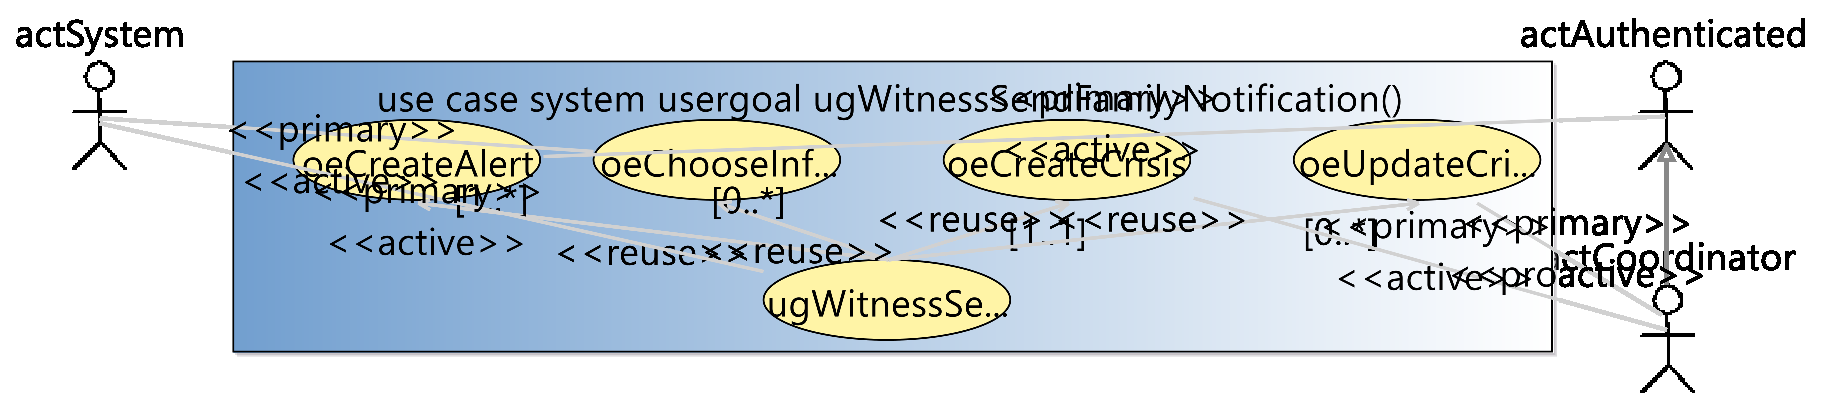
\includegraphics[
angle=0
,width=1.0\textwidth
]{./images-report-gen/usecase-model/usergoal/uc-ugWitnessSendFamilyNotification.eps}
\end{center}
\caption[lu.uni.lassy.excalibur.examples.icrash Use Case Diagram: uc-ugWitnessSendFamilyNotification]{Witness family notification}
\label{fig:lu.uni.lassy.excalibur.examples.icrash-RE-UCD-uc-ugWitnessSendFamilyNotification}
\end{figure}
\vspace{0.5cm}
